\chapter{Approach}\label{ch:approach}

In this chapter, we will provide a detailed explanation of the API and algorithm behind the concurrent range lock.

\section{Concurrent Range Lock API}\label{sec:api}

\begin{figure}[h]
    \centering
    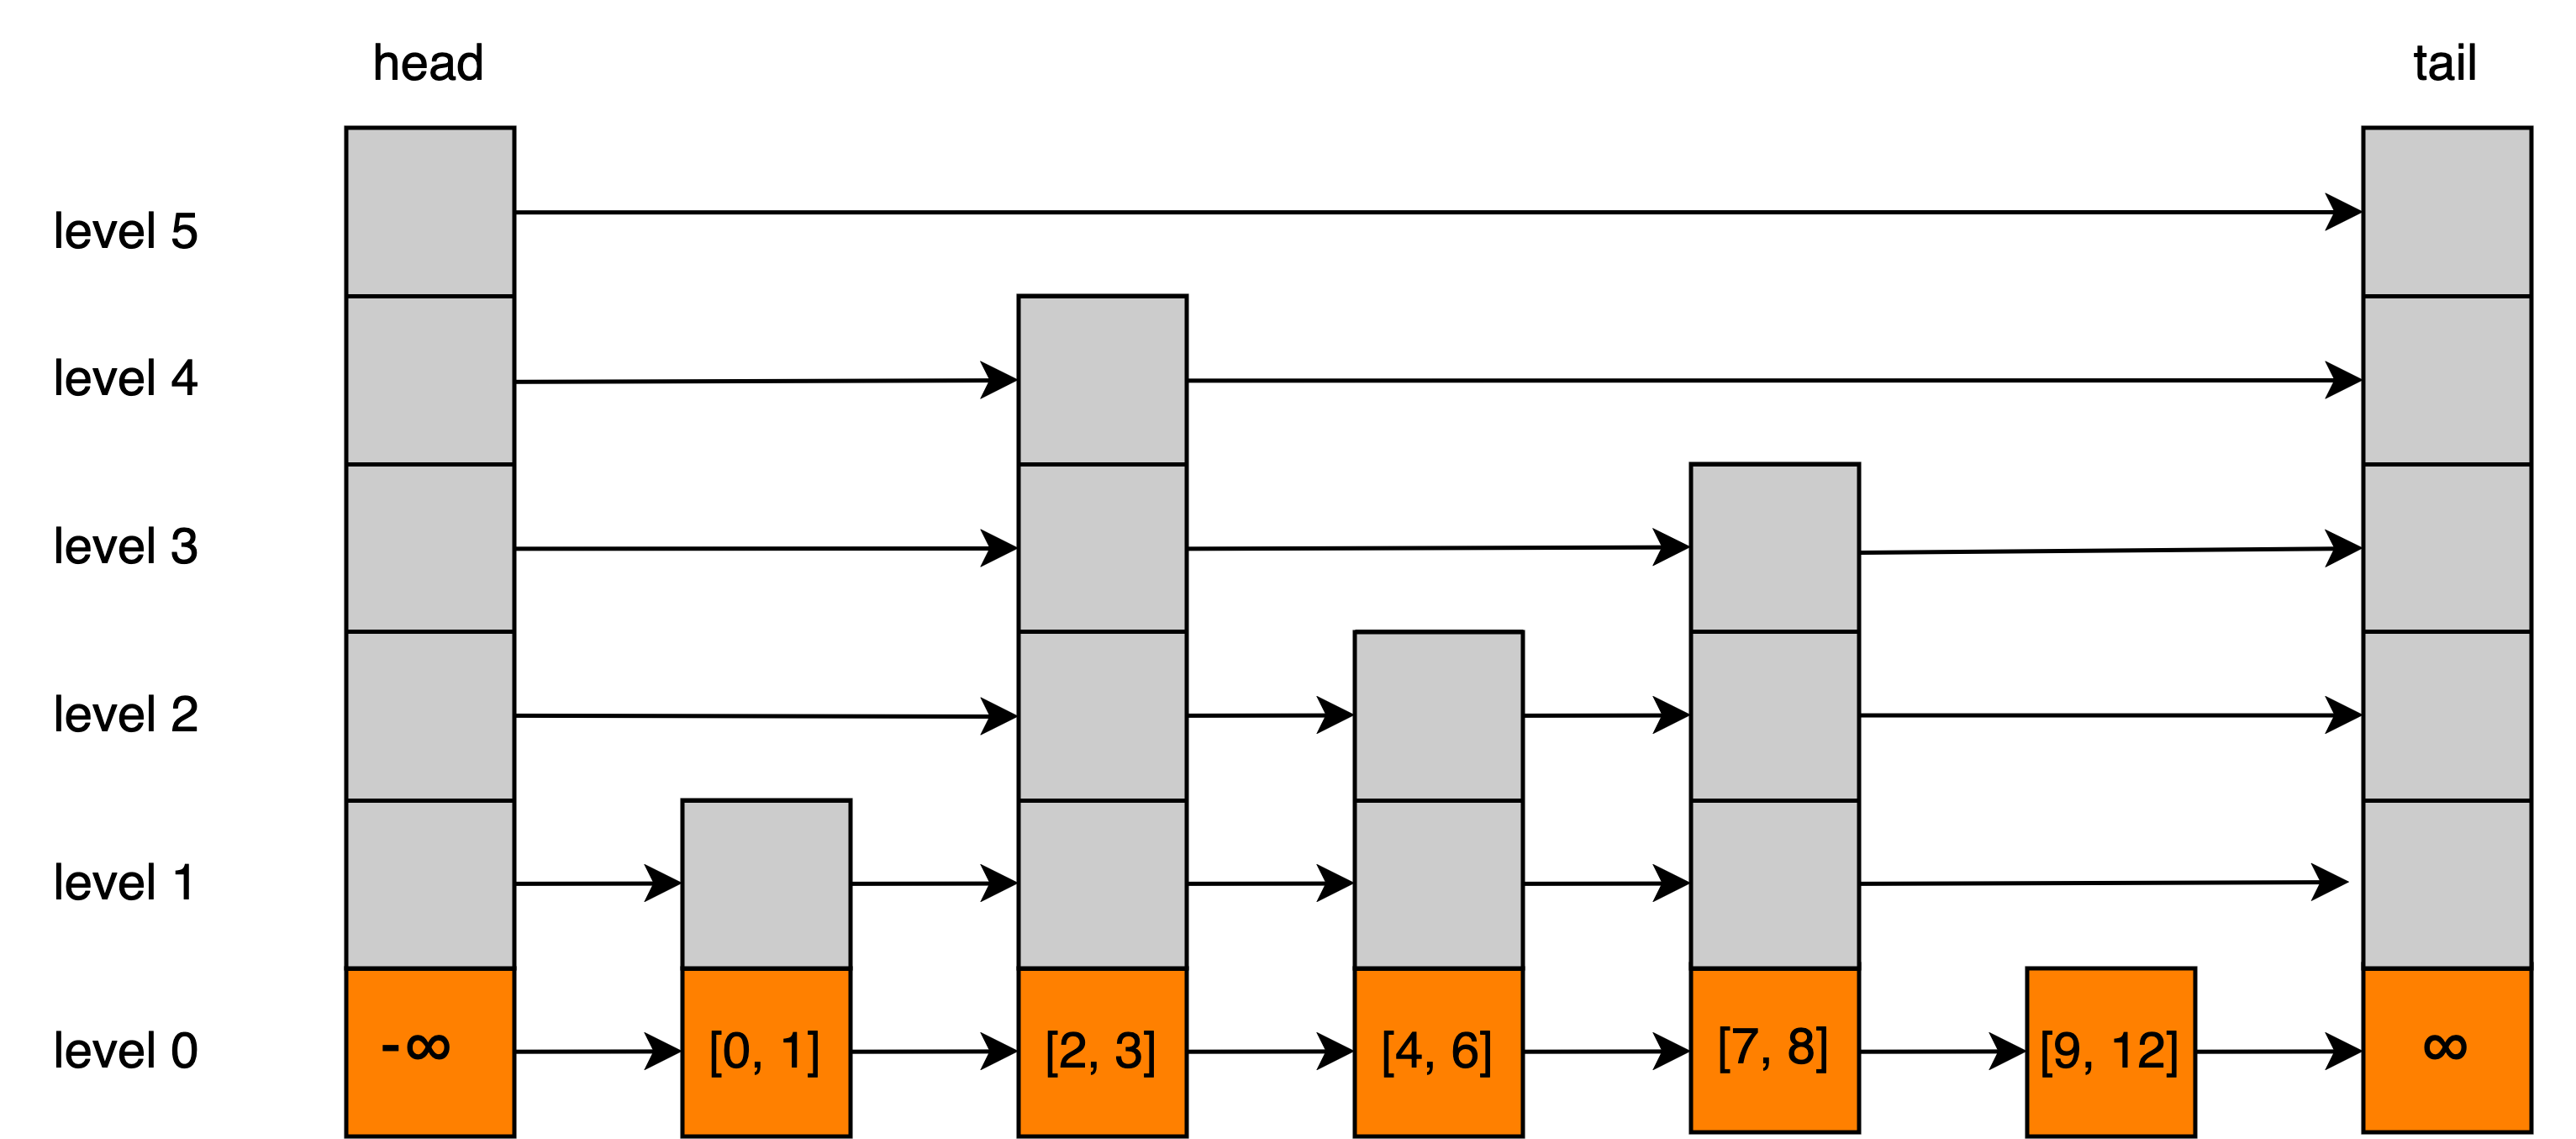
\includegraphics[width=0.8\textwidth]{./figures/rangelock.png}
    \caption{ConcurrentRangeLock. Each \texttt{Node} has a unique range.}
    \label{fig:concurrent_range_lock}
\end{figure}

The ConcurrentRangeLock class consists of two main functions: \texttt{tryLock} and \texttt{releaseLock}.

The \texttt{tryLock} method attempts to acquire a lock for the specified range \texttt{[start, end]}, returning \texttt{true} on success and \texttt{false} otherwise.
The \texttt{releaseLock} method releases the lock for the range \texttt{[start, end]}, with \texttt{true} indicating success and \texttt{false} if the range was not found or an error occurred.
We will discuss these methods in Subsection \ref{subsec:tryLock} and \ref{subsec:releaseLock}.

The two primary methods rely heavily on private searching methods such as \texttt{findInsert}, \texttt{findExact}, and \texttt{findDelete}, which handle insertion finding, exact range finding, and physical deletion of ranges, respectively. We will discuss these methods in Section \ref{subsec:find}.

\begin{figure}[h]
    \centering
    \lstinputlisting[style=mystyle,caption={Pseudocode for ConcurrentRangeLock API},label={lst:api}]{code/api.txt}
\end{figure}

\section{Life cycle}

Each thread has to call the \texttt{tryLock} method with the parameters range start, range end, thus the positions on the shared object that this thread wants to acquire. 
If there is no conflict, that is, if there is no overlap existing on the lock, \texttt{tryLock} is successful. Thread now has exclusive access to this segment of the shared object and can freely read and write this segment. After finish using this segment, thread can call \texttt{releaseLock} to return his access to this segment. If used correctly, \texttt{releaseLock} should always return true.

\begin{figure}[H]
    \centering
    
    \begin{tikzpicture}[->, auto, semithick, node distance=2cm]
    
    % Node styles
    \tikzstyle{thread1}=[state, draw=darkblue, line width=0.5mm, align=center]
    \tikzstyle{crl}=[draw=black, fill=none, minimum width=2cm, align=center]
    \tikzstyle{success1}=[state, draw=darkblue,line width=0.5mm, align=center]
    
    % Nodes
    \node[thread1] (worker1) {worker\_thread 1 \\ acquiring [0,512]};
    \node[crl,  right=2cm of worker1, yshift=-2cm] (crl) {Concurrent Range Lock};
    \node[success1, above=2cm of crl] (success1) {worker\_thread 1 \\ acquired [0,512]};
    \node[success1, right=9cm of worker1] (free1) {worker\_thread 1 \\ released [0,512]};

    % Numbers
    \node[above=0.2cm of worker1] {(1)};
    \node[above=0.2cm of success1] {(2)};
    \node[above=0.2cm of free1] {(3)};
    
    % Arrows and Labels
    \path[->] 
        (worker1) edge[draw=blue,bend left=10] node[left,yshift=-0.7cm] {tryLock(0,512)} (crl)
        
        (crl) edge[draw=blue,bend left=10] node[left] {success} (success1)
        
        (success1) edge[draw=darkblue,bend left=10] node[right] {releaseLock(0,512)} (crl)
        
        (crl) edge[draw=darkblue,bend right=20] node[right] {success} (free1);
    \end{tikzpicture}
    \caption{Life cycle of range lock}
    \label{fig:crl_life_cycle}
\end{figure}

\section{Algorithm in details}

For the sake of simplicity, we use \texttt{uint64\_t} for our pseudocode provided in this section. 
We use the template feature in our open-source C++ implementation to enable generic programming. 
For further detail, please refer to our \href{https://github.com/thuaduc/concurrent-range-locking}{open-source code}.

\begin{figure}[H]
    \centering
    \begin{tikzpicture}[->, auto, semithick, node distance=2cm]
    
    % Node styles
    \tikzstyle{thread1}=[state, draw=darkblue, line width=0.5mm, minimum width=1cm, minimum height=1cm, align=center]
    \tikzstyle{thread2}=[state, draw=darkred, line width=0.5mm, minimum width=1cm, minimum height=1cm, align=center]
    \tikzstyle{thread3}=[state, draw=darkgreen,line width=0.5mm, minimum width=2cm, minimum height=1cm, align=center]
    \tikzstyle{crl}=[draw=black, fill=none, minimum width=3cm, minimum height=1.5cm, align=center]
    \tikzstyle{success1}=[state, draw=darkblue,line width=0.5mm, minimum width=1cm, minimum height=1cm, align=center]
    \tikzstyle{success3}=[state, draw=darkgreen,line width=0.5mm, minimum width=1cm, minimum height=1cm, align=center]

    
    % Nodes
    \node[thread1] (worker1) {worker\_thread 1 \\ acquiring [0,512]};
    \node[thread2, below=1cm of worker1] (worker2) {worker\_thread 2 \\ acquiring [256, 1024]};
    \node[thread3, below=6cm of worker1] (worker3) {worker\_thread 3 \\ acquiring [1024,2048]};
    \node[crl,  right=4cm of worker2] (crl) {Concurrent Range Lock};
    \node[success1, right=4cm of worker1] (success1) {worker\_thread 1 \\ acquired [0,512]};    
    \node[success3, right=4cm of worker3] (success3) {worker\_thread 3 \\ acquired [1024, 2048]}; 

    % Numbers
    \node[left=0.2cm of worker1] {(1)};
    \node[left=0.2cm of worker2] {(2)};
    \node[left=0.2cm of worker3] {(3)};
    
    % Arrows and Labels
    \path[->] 
        (worker1) edge[draw=blue,bend left=10] node[left] {tryLock(0,512)} (crl)
        (worker2) edge[draw=red,bend left=10] node[above] {tryLock(256, 1024)} (crl)
        (worker3) edge[draw=darkgreen,bend left=10] node[right] {tryLock(1024, 2048)} (crl)
        (crl) edge[draw=blue,bend left=10] node[right] {success} (success1)
        (crl) edge[draw=red,bend left=10] node[below] {fail} (worker2)
        (crl) edge[draw=darkgreen] node[right] {success} (success3);
    \end{tikzpicture}
    \caption{The behavior of range lock case: three threads trying to lock ranges. Second thread failed because of overlap}
    \label{fig:crl_conflict}
\end{figure}

\subsection{Try Lock}\label{subsec:tryLock}

The \texttt{tryLock} method, shown in Listing \ref{lst:tryLock}, utilizes \texttt{findInsert()} to check if a node with the range \texttt{[start, end]} already exists. If found, \texttt{tryLock} returns \texttt{false}. 
Otherwise, it creates a new node and attempts to insert it into the list. 
The Node is inserted starting from the bottom level, with \texttt{compareAndSet()} ensuring the integrity of the insertion. 
If any insertion fails due to concurrent changes, \texttt{findInsert()} is called again to update the predecessors and successors, and the process repeats until successful.

\vspace{15pt}
\begin{figure}[h]
    \centering
    \lstinputlisting[style=mystyle,caption={Pseudocode for tryLock method},label={lst:tryLock}]{code/trylock.txt}
\end{figure}

\subsubsection*{Algorithm in details}
The \texttt{tryLock} method, shown in Listing \ref{lst:tryLock}, uses \texttt{findInsert()} to determine whether a node with range \texttt{[start, end]} is already in the list (line 7). 
\texttt{tryLock} also calls \texttt{findInsert()} to initialize the preds[] and succs[] arrays to hold the new Node's ostensible predecessors and successors.
If an unmarked node is found in the bottom-level list, \texttt{findInsert()} returns \texttt{true} and the \texttt{tryLock} method returns \texttt{false}, indicating that part of the target range is already acquired by other thread.
See Figure \ref{fig:crl_conflict} as an example.
The unsuccessful linearization point of \texttt{tryLock} is the same as the successful linearization point of \texttt{findInsert()} (line 8). 
If no node is found, the next step is to add a new node with the key into the structure.

A new node is created with a randomly chosen top-level (lines 10--11). 
The Node's next references are unmarked and set to the successors returned by the \texttt{findInsert()} method (lines 13--15).
The next step is to try to add the new Node by linking it into the bottom-level list between the \texttt{preds[0]} and \texttt{succs[0]} nodes returned by \texttt{findInsert()}. 
We use the \texttt{compareAndSet()} method to set the reference while validating that these nodes still refer one to the other and have not been removed from the list (line 17). 
If the  \texttt{compareAndSet()} fails, something has changed and the call restarts. 
If the  \texttt{compareAndSet()} succeeds, the item is added, and line 17 is the call's linearization point.
The {findInsert()} then links the Node in at higher levels (lines 21--25). 
For each level, it attempts to splice the Node by setting the predecessor, if it refers to the valid successor, to the new Node (lines 22--23). If successful, it breaks and moves on to the next level. 
If unsuccessful, then the Node referenced by the predecessor must have changed, and \texttt{findInsert()} is called again to find a new valid set of predecessors and successors (line 24). 
We discard the result of calling \texttt{findInsert()} because we care only about recomputing the ostensible predecessors and successors on the remaining unlinked levels. 
The method returns true once all levels are linked (line 27).

\subsection{Release Lock}\label{subsec:releaseLock}

The \texttt{releaseLock} method first calls \texttt{findExact()} to locate an unmarked node with the specified range \texttt{[start, end]}. 
If found, it marks all node levels except the bottom one, preparing the Node for removal. 
The method then attempts to mark the bottom-level link using \texttt{compareAndSet()}, which serves as the linearization point for a successful \texttt{releaseLock}. 
If marking fails due to concurrent modifications, the method retries or returns false, depending on the Node's state.

\vspace{15pt}
\begin{figure}[h]
    \centering
    \lstinputlisting[style=mystyle,caption={Pseudocode for releaseLock method},label={lst:releaseLock}]{code/releaselock.txt}
\end{figure}

\subsubsection*{Algorithm in details}

The \texttt{releaseLock} method, shown in Listing \ref{lst:releaseLock}, calls \texttt{findExact()} to determine whether an unmarked node with a matching range \texttt{[start, end]} is in the bottom-level list (line 7). 
If no node is found in the bottom-level list, or the Node with a matching range \texttt{[start, end]} is marked, the method returns false. 
The linearization point of the unsuccessful \texttt{releaseLock} is that of the \texttt{findExact()} method called in line 7. 

If an unmarked node is found, the method logically removes the associated key from the abstract set and prepares it for physical removal. 
This step uses the set of ostensible predecessors (stored by \texttt{findExact()} in \texttt{preds[]}) and the victim (returned from \texttt{findExact()} in \texttt{succs[]}). 
First, starting from the top-level, all links up to and \textbf{not including} the bottom-level link are marked (lines 12--20) by repeatedly reading next and its mark and applying \texttt{attemptMark()}. 
If the link is found to be marked (either because it was already marked or because the attempt succeeded), the method moves on to the next-level link. 
Otherwise, the current level's link is reread since another concurrent thread must have changed it, so the marking attempt must be repeated. 

Once all levels but the bottom one have been marked, the method marks the bottom level's next reference. 
If successful, this marking (line 27) is the linearization point of a successful \texttt{releaseLock}. 
The \texttt{releaseLock} method tries to mark the next field using \texttt{compareAndSet()}. 
If successful, it can determine that it was the thread that changed the mark from false to true. 
Before returning true, the \texttt{findDelete()} method is called. 
This call is an optimization: \texttt{findDelete()} physically removes all links to the Node it is searching for.

On the other hand, if the  \texttt{compareAndSet()} call fails, but the next reference is marked, then another thread must have concurrently removed it, so \texttt{releaseLock} returns false. 
The linearization point of this unsuccessful \texttt{releaseLock} is the linearization point of the \texttt{releaseLock} method by the thread that successfully marked the next field. 
Notice that this linearization point must occur during the \texttt{releaseLock} call because the \texttt{findExact()} call found the Node unmarked before it found it marked.

Finally, if the \texttt{compareAndSet()} fails and the Node is unmarked, the next Node must have changed concurrently. 
Since the victim is known, there is no need to call find() again, and \texttt{releaseLock} simply uses the new value read from next to retry the marking.

\subsection{Find}\label{subsec:find}

Both \texttt{tryLock} and \texttt{releaseLock} methods rely heavily on \texttt{find} methods.
There are several find methods in our implementation that serve different purposes:

\begin{itemize}
    \item \texttt{bool findInsert(uint64\_t start, uint64\_t end, Node** preds, Node** succs)}: checks if the target range \texttt{[start, end]} is free to be inserted.
    
    \item \texttt{bool findExact(uint64\_t start, uint64\_t end, Node** preds, Node** succs)}: checks if the target range \texttt{[start, end]} is already present in the skip list.
    
    \item \texttt{void findDelete(uint64\_t start, uint64\_t end)}: finds the target range \texttt{[start, end]} from the skip list to physically delete the Node which contains the corresponding range.
\end{itemize}

These \texttt{findInsert} and \texttt{findExact} methods also fill in the \texttt{preds[]} and \texttt{succs[]} arrays with the target node's predecessors and successors at each level.
Because the goal of \texttt{findDelete} is only to snip out all the deleted Node, there is no need to fill any array.

Nevertheless, these methods have to maintain the following two properties:

\begin{itemize}
    \item During traversal, they need to skip over marked nodes.
    They use \texttt{compareAndSet()} to ensure that they remove all softly deleted Node on the way.
    \item Every \texttt{preds[]} reference is to a node with a key strictly less than the target.
\end{itemize}

\vspace{15pt}

\begin{figure}[h]
    \centering
    \lstinputlisting[style=mystyle,caption={General pseudocode for find methods},label={lst:find}]{code/find.txt}
\end{figure}

\subsubsection{Algorithm in details}
The \texttt{find()} method starts by traversing the LockFreeSkipList from the \texttt{topLevel} of the head sentinel, which has the maximal allowed node level.
It proceeds down the list level by level, filling in the \texttt{preds} and \texttt{succs} nodes.
These nodes are repeatedly advanced until \texttt{pred} refers to a node with the \texttt{end} value on that level that is strictly less than the target range \texttt{end} (lines 13--29).

While traversing, it repeatedly snips out marked nodes from the current level as they are encountered (lines 15--22) using a \texttt{compareAndSet()}.
\texttt{compareAndSet()} function also validates that the next field of the predecessor still references the current Node.

Once an unmarked \texttt{curr} node is found (line 23), it is tested to see if its \texttt{start} is greater than or equal to the target \texttt{start}.
If so, \texttt{pred} is advanced to \texttt{curr}, \texttt{curr} is advanced to \texttt{succ}, and the traverse continues.
Otherwise, the current range of \texttt{pred} is the immediate predecessor of the target node.
The \texttt{find()} method then breaks out of the current level search loop, saving the current values of \texttt{pred} and \texttt{curr} (lines 26--32).

The \texttt{find()} method continues this process until it reaches the bottom level.
An important point is that each level's traversal maintains the previously described properties.
Specifically, if a node with the target key is in the list, it will be found at the bottom level even if nodes are removed at higher levels.
When traversal stops, \texttt{pred} refers to a predecessor of the target node.
The method descends to each next lower level without skipping over the target node.
If the Node is in the list, it will be found at the bottom level.
Additionally, if the Node is found, it cannot be marked because if it were marked, it would have been snipped out in lines 15--22.
Thus, the condition test on line 35 only needs to check if there are overlap ranges (\texttt{findInsert}) or if the start and end of the Node match the target start and end (\texttt{findExact}).
\begin{enumerate}
    \item \texttt{findInsert}:
    \begin{lstlisting}[style=nonum, label={}]
 return (!(start > pred->getEnd() && end < curr->getStart()));
    \end{lstlisting}
    \item \texttt{findExact}:
    \begin{lstlisting}[style=nonum, label={}]
 return (start == curr->getStart() && end == curr->getEnd());
    \end{lstlisting}
\end{enumerate}

The linearization points for both successful and unsuccessful calls to the \texttt{find()} method occur when the \texttt{curr} reference at the bottom-level list is set, either at line 11 or line 20, for the last time before the success or failure of the \texttt{find()} call is determined at line 35.
